\section{Supplementary figures}
\label{app:supplementary_figures}

% Supplementary figures reserved for additional versions that may be moved
% out of the main text in a later shortened submission draft.
% Candidates: full top-eigenvector loading figure, original MST/PMFG rough
% comparison figures, selected body figures after narrative shortening.

Additional figures and tables generated by the computational workflow are retained as supplementary material. These include asset-universe tables, return summaries, correlation matrices, RMT eigenvector loadings, network edge lists, clique lists, centrality rankings and detailed forecasting results by asset, horizon, model and feature set.

\begin{center}
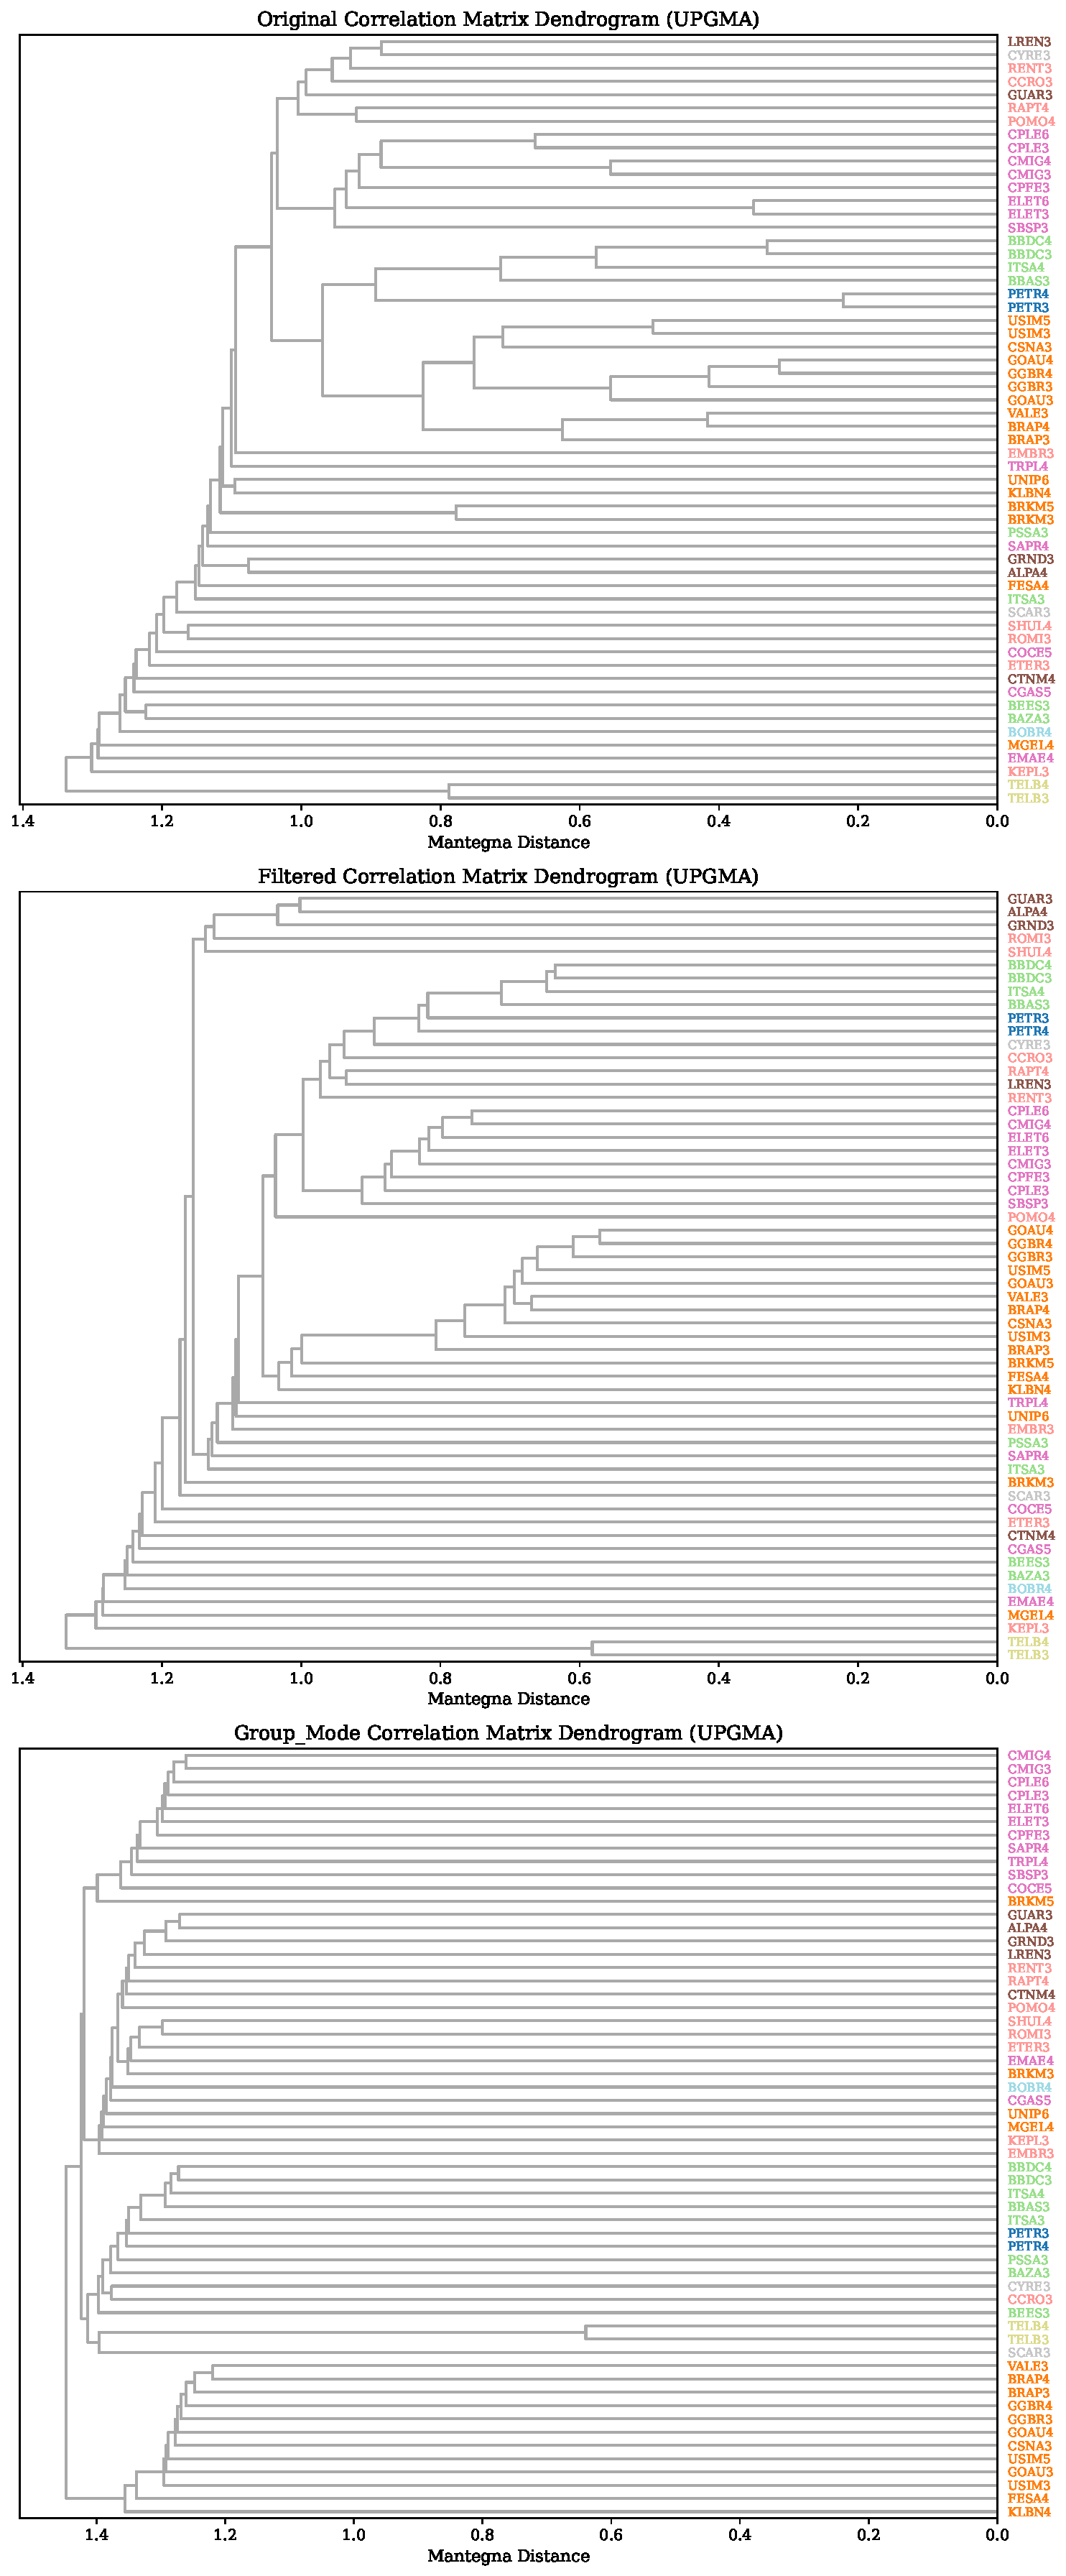
\includegraphics[width=\linewidth,height=0.90\textheight,keepaspectratio]{images/figure_9_dendrograms_comparison.pdf}
\captionof{figure}{Full dendrogram comparison for original, filtered and group-mode matrices using Mantegna distances and average linkage. The main text presents the group-mode tree only, together with the cophenetic summary.}
\label{fig:dendrograms_full_supplement}
\end{center}

\begin{center}
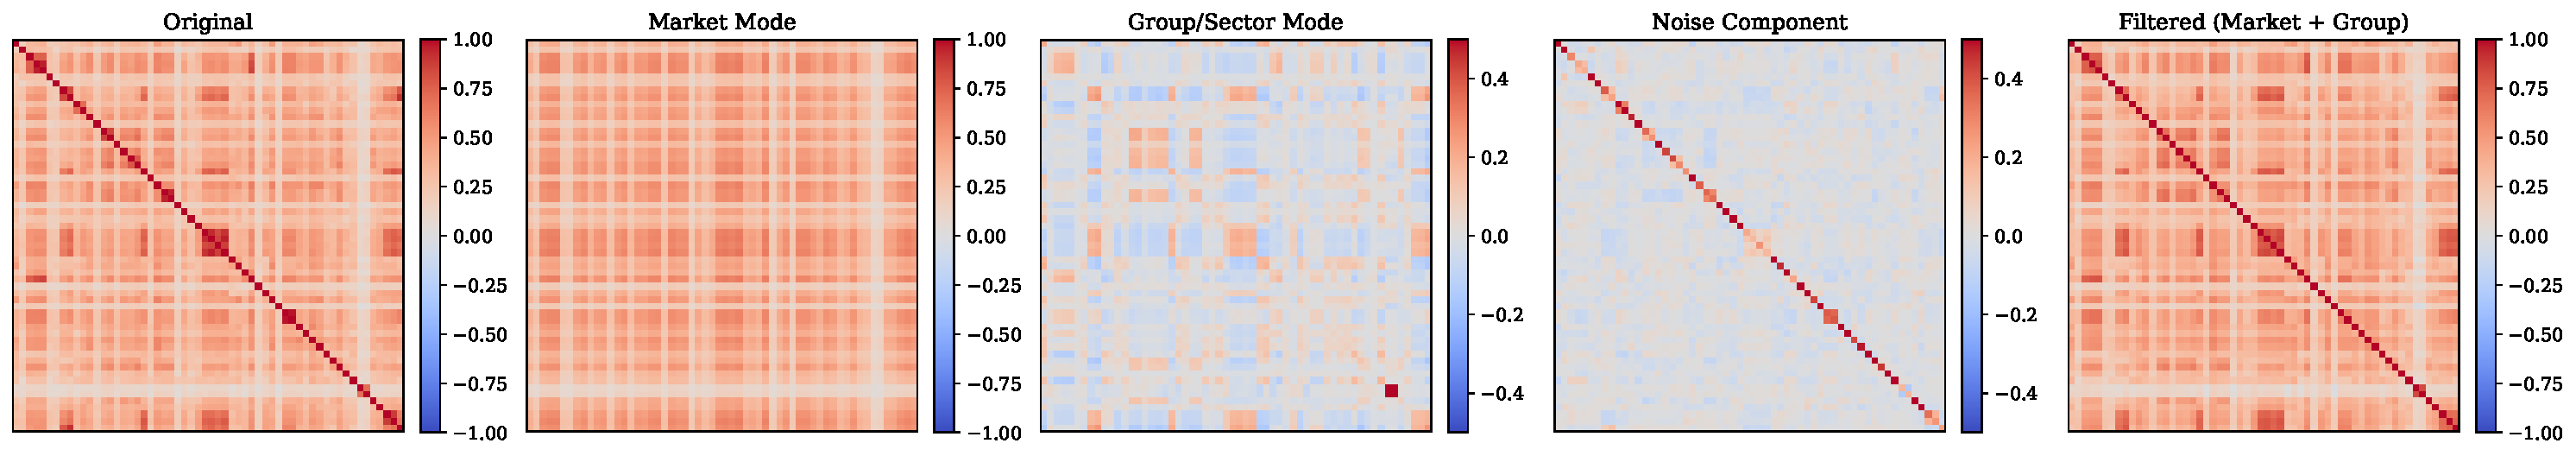
\includegraphics[width=\linewidth]{images/figure_8_rmt_filtered_matrices.pdf}
\captionof{figure}{Full RMT decomposition: original correlation, market-mode, candidate group/sector, noise-compatible and retained components. The main text presents the original and group/sector panels at readable scale.}
\label{fig:rmt_full_components_supplement}
\end{center}
